\chapter{Project Plan}
This chapter will discuss what needs to be done for the project to be successful, the paths that can be taken, areas that can be explored as an extension and fall-back positions in the limit of time.
\par
\section{The Artifact}
The key aim of the project is to produce a code artifact that can verify the correctness of Elixir programs. "Verify" is being used as an umbrella term for three potential components of the artifact. In no particular order:
\begin{itemize}
    \item Determining if a program is deadlock-free.
    \item Allowing users to write specifications about functions that are inline and verifiable.
    \item Verifying liveness properties. 
\end{itemize}
It would be difficult/infeasible to design a tool that can do all three from scratch and similarly, I have yet to find a tool that can do all three. Hence, my current path forward is to use a combination of existing tools where necessary to achieve these verification feats. The most appropriate tools I have identified for each case respectively are the SPIN model-checker, the Boogie IVL for theorem-proving and the TLC model-checker.
\par
Given these three tools, the plan would be to develop a command-line tool, that takes an Elixir project as an input, parses the Elixir code, and extracts the underlying model from the project to create an internal representation that can be used to generate models in the three target output grammers.
\par
The main difficulty of this project will lie in the design of Elixir. Elixir focuses on the concurrent execution of programs, using the actor model for communication between sequential processes executing in parallel. None of the target output tools have support for message passing and Boogie does not support concurrency. That means the main challenge of the project will be designing a framework for modelling programming languages that use message-passing as a first-class solution to communication. If the framework is well designed, this may not be limited to Elixir, the intermediate representation could be a target grammar that any message-passing oriented language can be translated into (such as Rust). However, for the scope of this project, modelling Elixir will be sufficient.
\par
Once a model has been extracted from an Elixir program, the next step will be code generation for the relevant tools, which can then be ran to determine the correctness of the program.
\section{Timeline and Milestones}
This section is a brief overview of what needs to happen and what has already began.
\subsubsection{Manual Translation (started)}
The first step involved understanding what an Elixir program looks like in the target representations. I spent time taking some basic Elixir programs and translating them into Promela (the specification language used by SPIN) to gather an understanding of how they can begin to be translated. I modelled four programs, an entirely sequentially executed program, a program that introduces a deadlock, a program that introduces a livelock and a program based on a deadlocking dining philosophers algorithm. While doing this, I made notes of how various components can be modelled in Promela as well as what is difficult to model. A brief summary of some findings:
\begin{itemize}
    \item In the basic deadlock model, a deadlock was detected.
    \item In the dining philosophers model (a more complex example of an Elixir program) a deadlock was detected.
    \item In the basic livelock model, the model-checker ran forever and did not detect the livelock. In theory, Promela should be detecting livelocks so more investigation needs to be done into how models need to be bound to allow for the successful detection.
    \item The key primitives unique to the actor model were able to be modelled with fair success in Promela.
\end{itemize}
As well as translating Elixir programs to Promela models, I spent some important time translating quoted expressions (equivalent to ASTs) to models, as Elixir provides the functionality to easily access them.
\subsubsection{Parsing (started)}
Parsing Elixir programs so they can be stored in an intermediate representation is important. Because of the access to quoted expressions, there is no need to parse Elixir grammar directly, instead parsing quoted expressions is easier. They are guaranteed to be well-formed, and when parsed you are left with an AST by nature. Work has begun here using a parser combinator library (pest) in Rust. The Elixir developers do not provide exhaustive documentation of the grammar of quoted expressions, so instead they have to be derived from examples and trial-and-error.
\subsubsection{Model Extraction (started)}
The main challenge of the project is model extraction. It introduces many questions that need answering:
\begin{itemize}
    \item What does a sequential execution of statements look like?
    \item How can functions be represented to be modelled in specifications that don't support functions (Promela)?
    \item How can Elixir recursion be modelled in specifications that don't support recursion (Promela)?
    \item How can concurrency processes be modelled as a sequential process (Boogie)?
    \item How can message-passing be modelled, in particular when specifications don't support shared memory?
\end{itemize}
Unfortunately, the list goes on the more you look into the Elixir language. A starting point will be modelling sequential programs.
\subsubsection{Promela code-gen (begin in term 2)}
The first model checker I aim to target is Promela. Although it doesn't natively support function calls or definitions it does support concurrency, therefore I deem it an easier milestone to reach. Once code-gen for Promela is implemented, it should be possible to begin proving Elixir programs are deadlock-free, which is a massive step towards being a verification-aware language.
\begin{figure}[h]
    \centering
    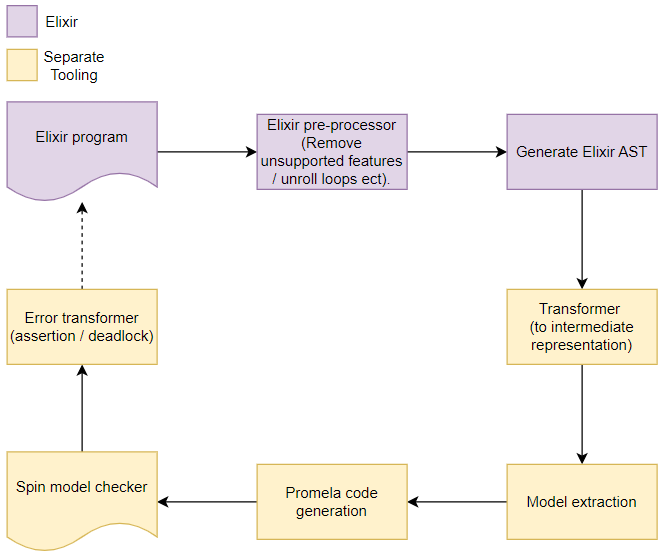
\includegraphics[width=0.6\textwidth]{images/system_design_v0.png}
    \caption{v0 system design for deadlock detection.}
    \label{fig:v0_system_design}
\end{figure}
\subsubsection{Extending Elixir with Metaprogramming (begin in term 3)}
It will be difficult within the scope of the project to allow any Elixir program without modification to be verified. Using metaprogramming, steps can be taken to introduce an Elixir library that allows developers to write code that is easier to verify. For example, developers can introduce bounds to mailboxes and recursive calls that make model extracting a lot more direct. Anything unbounded won't be verifiable, so I want to put the burden on the developer writing specifications instead of the artifact to approximate bounds.
\par
Metaprogramming can also be used to introduce pre- and post-conditions to Elixir to extend the support for verification.
\subsubsection{Boogie code-gen (term 3 / future work)}
After extending the Elixir language to allow the introduction of pre- and post-conditions, code-gen for Boogie programs can take place that allows stronger verification support for Elixir. I deem this an important part of the project but it depends on a lot of prior work being finished, so it's hard to determine if it fits on the timeline.
\subsubsection{Liveness (future work)}
It is unlikely that liveness will be implemented as part of the verification toolkit unless it is discovered one of the existing downstream tools supports it. I believe code-gen for a new tool will be required (such as TLA+) to achieve this, which is likely to be infeasible in the scope of the project, but on my radar.